\documentclass{scrartcl}
\usepackage[a4paper,top=2cm,bottom=2.5cm,left=2.5cm,right=2.5cm,marginparwidth=0cm]{geometry}
\usepackage[english]{babel}
\usepackage[linguistics]{forest}

\usepackage[
    doi=true,
    language=english,
    natbib=true,
    sortcites,
    style=unified,
    useprefix=true,
    ]{biblatex}


% Fonts, languages
\usepackage[warnings-off={mathtools-colon, mathtools-overbracket}]{unicode-math}
\usepackage{fontspec}
\defaultfontfeatures{Ligatures=TeX}
\usepackage[sb]{libertinus-otf}
\usepackage[scale=MatchLowercase]{FiraMono}
\usepackage{fontawesome5}

% Nicer tables
\usepackage{booktabs}
\usepackage[table]{xcolor}
\usepackage{colortbl}
\usepackage[nopatch=footnote]{microtype}
\usepackage{tabularx}
\usepackage{longtable}
\usepackage{float}
\usepackage[section]{placeins}
\usepackage{booktabs}
\usepackage{multirow}
\usepackage{array}

\usepackage[unicode,hidelinks]{hyperref}
\usepackage[normalem]{ulem} % for strikethrough \sout

\usepackage{scrlayer-scrpage}
\newpairofpagestyles{titlepage}{%
    \setkomafont{pageheadfoot}{%
        \small\normalfont 
    }
    \rohead{}
    \lohead{}
}
\pagestyle{scrheadings}
\setkomafont{pagenumber}{\footnotesize}%\sffamily}
\setkomafont{pageheadfoot}%
    {\small\addfontfeature{LetterSpace=10,Numbers=OldStyle}\scshape\sffamily}
\clearpairofpagestyles{}
\cfoot[\pagemark]{\pagemark}
% \rohead{\MakeLowercase{\emph{\shorttitle}}}
%\lohead{\MakeLowercase{\authorlast}}


% Titlepage
\setkomafont{author}{\large\sffamily}


% Chapter/section headings
\setcounter{secnumdepth}{3}

% Linguistics
\usepackage{langsci-gb4e}
\newcommand{\judgement}[1]{\makebox[0pt][r]{#1}}



\usepackage{cleveref}
\usepackage{enumitem}

%% Line breaks
\widowpenalty=10000
\clubpenalty=10000

% useful 
\usepackage{orcidlink}
\newcommand{\email}[1]{\href{mailto:#1}{#1}}

% copyright notice at end
\usepackage[framemethod=TikZ]{mdframed}
\newenvironment{ccnotice}[1]{%
    \begin{mdframed}[%
        linewidth=0pt,
        leftmargin=1pt,
        rightmargin=1pt,
        backgroundcolor=gray!10!white,
        font=\sffamily,
    ]\relax%
}{\end{mdframed}}


\usepackage[autostyle=true,english=american]{csquotes}
\renewcommand*{\mkccitation}[1]{ (#1)}

\usepackage{xcolor}
\usepackage{titlesec}
\definecolor{mycolor}{HTML}{2e6a1e}
\titleformat{\section}
              {\normalfont\Large\bfseries\color{mycolor}} % Formatting
              {\thesection}            % Label
              {2em}                   % Space after label
              {}  
\titleformat{\subsection}{\normalfont\large\bfseries\color{mycolor}}{\thesubsection}{1.2em}{} 
\titleformat{\subsubsection}{\normalfont\normalsize\bfseries\color{mycolor}}{\thesubsubsection}{1em}{} 
\titleformat{\paragraph}
  {\normalfont\normalsize\bfseries}{\theparagraph}{1em}{}


% title page

\title{\fulltitle}
\date{}


\urlstyle{same}

\usepackage{svg}
\usepackage{amsmath}

\usepackage{pdflscape}

\hypersetup{
    colorlinks=false,
    linkcolor=blue,
    filecolor=magenta,      
    urlcolor=cyan,
    pdftitle={Deliverable-D4-Gruppo3},
    pdfpagemode=FullScreen,
    }
\newcommand{\fulltitle}{
                        \includesvg[width=0.6\linewidth]{../Logo/AgriTrentoSlogan.svg} \\
                        \vspace{3.4cm}
                        \color{mycolor}Deliverable D4 - Gruppo 3
                        }


\newenvironment{objitem}{
    \begin{enumerate}
    \renewcommand{\labelenumi}{\textbf{O\arabic{enumi}}}
}
{\end{enumerate}}

\newenvironment{rfenum}{
    \begin{enumerate}
    \renewcommand{\labelenumi}{\textbf{RF\arabic{enumi}}}    
    \renewcommand{\labelenumii}{RF\arabic{enumi}.\arabic{enumii}}
    \renewcommand{\labelenumiii}{RF\arabic{enumi}.\arabic{enumii}.\arabic{enumiii}}
    
}
{\end{enumerate}}

\newenvironment{rnfenum}{
    \begin{enumerate}
    \renewcommand{\labelenumi}{\textbf{RNF\arabic{enumi}}}    
    \renewcommand{\labelenumii}{RNF\arabic{enumi}.\arabic{enumii}}
    \renewcommand{\labelenumiii}{RNF\arabic{enumi}.\arabic{enumii}.\arabic{enumiii}}
}
{\end{enumerate}}

\newenvironment{attori}{
    \begin{enumerate}
    \renewcommand{\labelenumi}{\textbf{2.\arabic{enumi}}}    
    \renewcommand{\labelenumii}{2.\arabic{enumi}.\arabic{enumii}}
    \renewcommand{\labelenumiii}{2.\arabic{enumi}.\arabic{enumii}.\arabic{enumiii}}
}
{\end{enumerate}}


\author{
    \href{https://www.linkedin.com/in/cristianoberardo/}{Cristiano Berardo} - 234428 - \href{https://github.com/CristianoBerardo}{\footnotesize \faGithub \ GitHub}\\
    \href{https://www.linkedin.com/in/martina-de-piccoli-957602353/}{Martina De Piccoli} - 235165 - \href{https://github.com/martinadep}{\footnotesize \faGithub \ GitHub}\\
    \href{https://www.linkedin.com/in/giacomo-vettore-62b571233/}{Giacomo Vettore} - 240396 - \href{https://github.com/giacomovettore02}{\footnotesize \faGithub \ GitHub}\\
}

% --------------- Start Document  -----------------------------

\begin{document}


\maketitle
\thispagestyle{titlepage}

\begin{center}

    \href{https://github.com/CristianoBerardo/Progetto-Ingegneria-del-Software}{ \faGithub \ \Large Progetto-Ingegneria-del-Software repository GitHub}
    
    \vspace{0.25cm}
    \href{https://agritrento.docs.apiary.io/}{\faLink \ \Large agritrento.docs.apiary.io}
    
    \vspace{0.25cm}
    \href{https://agritrento-rhzf.onrender.com}{\faLink \ \Large agritrento-rhzf.onrender.com}

    \vspace{0.25cm}
    \href{https://agritrento.onrender.com/api}{\faLink \ \Large agritrento.onrender.com/api (BE)}
    
    \vspace{0.25cm}
    \href{https://stats.uptimerobot.com/udFxPl75LM/800696152}{\faLink \ \Large Monitor Up-Time Backend}
    
    % \vspace{5.4cm}

\vspace{0.5cm}
\underline{\textbf{NOTA IMPORTANTE: se non vengono visualizzati i prodotti bisogna triggerare }} \\
\underline{\textbf{\href{https://agritrento.onrender.com/api}{agritrento.onrender.com/api}}}

\end{center}
\vspace{1.1cm}
% \begin{table}[h!]
%     \centering
%     \begin{tabular}{c|c|c}
%         Nome utente & Password & Note\\
%         \hline
%         cliente@cliente.it & cliente@cliente.it & \\
%         produttore@produttore.it &  produttore@produttore.it & \\
%         amministratore@amministratore.it&  amministratore@amministratore.it & \\
%     \end{tabular}
% \end{table}


\begin{table}[h!]
    \renewcommand{\arraystretch}{1.2} 
    \centering
    \begin{tabular}{c|c|c}
        \textbf{Ruolo} & \textbf{Nome utente e Password} & \textbf{Note}\\
        \hline
        Cliente & cliente@cliente.it & Nuovo account\\
        Produttore& az1@gmail.com & Sono già presenti alcuni prodotti\\
        Amministratore & admin@admin.it & Puramente UI
    \end{tabular}
\end{table}

\vspace{1.7cm}
\begin{abstract}
    \centering
    \noindent
    \textbf{Idea di progetto:} \textit{sviluppare una piattaforma web che faciliti la prenotazione e la vendita di frutta e verdura del mercato contadino di Trento, incentivando il consumo di prodotti stagionali locali, favorendo pratiche sostenibili e nel rispetto del nostro territorio.}
\end{abstract}


\section*{Strategia di Branching}

Per la gestione del codice sorgente di questo progetto, adotteremo la strategia di branching \textbf{Feature Branch Workflow}.
Ogni nuova funzionalità verrà sviluppata in un branch dedicato, \verb|feature branch|, creato a partire dal branch principale, \verb|main|, sempre aggiornato.

Al completamento, il codice viene sottoposto a revisione tramite \textit{pull request} e, solo dopo approvazione, integrato nel branch main.

Questo approccio garantisce stabilità e qualità del codice durante lo sviluppo incrementale previsto dalla metodologia SCRUM.

\section*{Product backlog}

\vspace{-1cm}

\renewcommand{\arraystretch}{2} 
\begin{center}
\centering
\begin{longtable}{
  >{\centering\arraybackslash}p{0.5cm}|
  >{\raggedright\arraybackslash}m{2.7cm}|
  >{\raggedright\arraybackslash}m{3.5cm}|
  >{\centering\arraybackslash}p{1.2cm}|
  >{\centering\arraybackslash}p{0.9cm}|
  >{\centering\arraybackslash}p{0.9cm}|
  >{\raggedright\arraybackslash}m{3.5cm}
}
  \caption{Tabella Product Backlog }\label{tab:ProductBackLogTable}\\
  \hline
  ID & Nome & User Story & Priorità & Story & Impor &How \\
     &      & &          &points &tanza  & to demo\\
  \hline
  \endfirsthead

  \hline
  ID & Nome & User Story& Priorità & Story & Impor &How \\
     &      & &          &points &tanza  & to demo\\
  \hline
  \endhead

  29 & Creazione database
     & Come team, dobbiamo creare un database, così da poter memorizzare i dati richiesti
     & Critica  & 3   & 433  & Accedere con username e password al portale di mongoDB \\
  31 & Creazione repository GitHub
     & Come team, dobbiamo creare una repo GitHub e inizializzarla, in modo da facilitare lo sviluppo dell'applicazione
     & Critica  & 5   & 260  & Visionare la presenza della repo su GitHub dai link sopra riportati \\
  14 & Inserimento prodotto
     & come produttore, vorrei poter aggiungere un nuovo prodotto con descrizione, quantità e prezzo, così da metterlo in vendita sulla piattaforma
     & Critica  & 13  & 100  & Il produttore troverà un form dove inserire i prodotti \\
  15 & Rimozione prodotto
     & come produttore, vorrei poter rimuovere un prodotto dalla lista, così da non renderlo più disponibile per l'acquisto
     & Bassa    & 3   & 100  &  Il produttore troverà un'icona cestino o una scritta da cliccare per eliminare il prodotto\\
  20 & Aggiornamento prodotto
     & come produttore, vorrei poter aggiornare le informazioni di un prodotto esistente, come prezzo, descrizione e quantità, così da mantenere l'offerta aggiornata
     & Alta     & 8   & 100  &  Il produttore troverà un'icona matita o una scritta da cliccare per aggiornare il prodotto\\
  2  & Autenticazione cliente/produttore
     & come cliente/produttore, vorrei potermi autenticare per accedere ai miei dati salvati
     & Critica  & 21  & 61   &  L'utente troverà un bottone di login per accedere alla piattaforma\\
  30 & Servizio di autenticazione
     & Come team, dobbiamo creare e capire come funziona Google OAuth, così da permettere il SSO e la gestione degli account
     & Critica  & 21  & 61   &  Visionare se è stato implementato il bottone che permetta di autenticarsi con Google\\
  32 & Studiare i framework e tool necessari
     & Come team, dobbiamo capire meglio come utilizzare al meglio i framework e tool, così da realizzare al meglio l'applicazione
     & Critica  & 21  & 61   &  Visionare il lavoro svolto durante i due sprint\\
  16 & Visualizzazione prodotti
     & come produttore, vorrei poter visualizzare la lista dei prodotti che ho già aggiunto, così da gestire facilmente il mio inventario
     & Alta     & 13  & 61   & Il produttore troverà uno spazio dedicato, intera pagina o una parte di essa, dove poter visualizzare tutti i prodotti messi a disposizione \\
  18 & Notifica ordini
     & come produttore, vorrei ricevere una notifica quando viene effettuato un ordine, così da poterlo gestire tempestivamente
     & Alta     & 13  & 61   & Dopo che un utente ha effettuato un ordine deve ricevere una notifica via mail dell'ordine da preparare \\
  10 & Conferma ordine
     & come cliente, vorrei ricevere una conferma d'ordine con i dettagli, il metodo di pagamento e le istruzioni per il ritiro, così da sapere che il mio ordine è stato registrato
     & Media    & 13  & 38   &  Dopo aver pagato l'ordine al cliente verrà inviata una mail con la conferma e il riepilogo dell'ordine \\
  26 & Gestione segnalazioni
     & come amministratore, vorrei poter ricevere e gestire segnalazioni di problemi o anomalie dagli utenti, così da risolvere rapidamente eventuali disservizi
     & Media    & 13  & 38   & Creare una segnalazione e verificare che questa venga ricevuta come mail dall'amministartore \\
  1  & Registrazione cliente/produttore
     & come cliente/produttore, vorrei potermi registrare nell'applicazione, per salvare i miei dati
     & Critica  & 34  & 38   &  Dopo aver compilato il form di registrazione, provare a fare il logout e successivamente il login e vedere se i dati sono rimasti\\
  5  & Ricerca prodotti
     & come cliente, vorrei poter cercare prodotti usando parole chiave e filtri per categoria, prezzo e disponibilità, così da trovare facilmente ciò che mi serve
     & Critica  & 34  & 38   & Provare a ricercare utilizzando la barra ricera presente nella home page e verificare la correttezza dei risultati \\
  4  & Recupero password
     & come cliente/produttore, vorrei poter recuperare la password del mio account
     & Alta     & 21  & 38   & Durante il login cliccare il pulsante recupera password e seguire le istruzioni e verificare se la password viene effettivamente cambiata\\
  7  & Visualizza dettaglio
     & come utente, vorrei poter visualizzare il dettaglio di un prodotto (Descrizione, prezzo e disponibilità)
     & Bassa    & 8   & 37   & Verificare se esiste una schermata che permetta all'utente di visualizzare i prodotti \\
  3  & Eliminazione cliente/produttore
     & come cliente/produttore, vorrei poter eliminare il mio account
     & Media    & 21  & 23   &  Nella pagina dedicata al profilo dovrà comparire un bottone "elimina account" che se cliccato elimina tutti i dati relativi a quell'account\\
  9  & Checkout ordine
     & come cliente, vorrei poter concludere il processo di checkout con un riepilogo dettagliato dell'ordine, così da verificare tutte le informazioni prima della conferma
     & Media    & 21  & 23   & Prima della transazione economica si deve visualizzare una schermata di riepilogo oridne \\
  17 & Visualizza ordini
     & come produttore, vorrei poter visualizzare gli ordini effettuati presso la mia azienda agricola, così da poterli preparare ed evadere entro le scadenze.
     & Media    & 21  & 23   &  Verificare che nella schermata del produttore sia presente una pagina, o parte di essa, predisposta per la visualizzazione degli ordini effettuati dai clienti\\
  8  & Aggiunta al carrello
     & come cliente, vorrei poter scegliere i prodotti desiderati e specificare le quantità da aggiungere al carrello, così da preparare il mio ordine
     & Alta     & 34  & 23   & Cercare un prodotto desiderato e selezionare aggiunti al carrello specificando la quantità \\
  22 & Gestione promozioni
     & come produttore, vorrei poter impostare promozioni e sconti temporanei sui prodotti, così da incentivare gli acquirenti ad acquistare di più
     & Bassa    & 13  & 23   &  Verificare che il produttore possa inserire sconti ai prodotti sia non ancora inseriti che inseriti in precedenza\\
  27 & Monitoraggio performance
     & come amministratore, vorrei avere strumenti per monitorare in tempo reale le performance dell'applicazione e i flussi di traffico, così da individuare e gestire anomalie
     & Bassa    & 21  & 14   &  Nella schermata amministratore si dovrà avere una dashboard dove quando un cliente ha fatto un ordine si aggiorni nel giro di qualche minuto\\
  6  & Ricerca produttore
     & come utente, vorrei poter cercare un produttore dalla lista per accedere al suo catalogo di prodotti
     & Media    & 55  & 9    & Nella schermata verrà visualizzata una barra di ricera del produttore verificare se questa funzioni \\
  11 & Cronologia ordini
     & come cliente, vorrei poter accedere a una sezione “I miei ordini” per visualizzare la cronologia degli ordini effettuati, con dettagli e stato aggiornato
     & Bassa    & 55  & 5    & Verificare se è presente una sezione "I miei ordini" e che essa contenga lo storico \\
  13 & Recensioni prodotti
     & come cliente, vorrei poter lasciare recensioni e valutazioni sui prodotti acquistati, così da condividere la mia esperienza con gli altri utenti
     & Minore   & 55  & 3    &  Provare ad inserire una recensione dei prodotti e verificare che essa compaia\\
  12 & Esegui pagamento online
     & come cliente, vorrei poter pagare il mio ordine direttamente sulla piattaforma, così da velocizzare il ritiro
     & Bassa    & 89  & 3    &  Provare ad eseguire un ordine di pagamento online \\
  19 & Ricevi pagamento online
     & come produttore, vorrei poter ricevere pagamenti digitali sicuri in anticipo, così da essere certo di ricevere il pagamento prima della consegna
     & Bassa    & 89  & 3    &  Verificare che il produttore possa accettare il pagamento anticipato della merce\\
  24 & Gestione account
     & come amministratore, vorrei poter visualizzare, modificare e gestire tutti gli account registrati, così da mantenere il controllo sugli utenti della piattaforma
     & Bassa    & 89  & 3    & Nella scheda dedicata verificare se compare la possibilità di modifica, eliminazione di un account \\
  21 & Dashboard statistiche
     & come produttore, vorrei poter consultare una dashboard con statistiche su vendite e ordini, così da monitorare l'andamento della mia attività
     & Minore   & 89  & 2    &  Verificare la presenza di una pagina dedicata con le statistiche di vendita \\
  28 & Generazione report
     & come amministratore, vorrei poter generare report aggregati su vendite, ordini e statistiche d'uso della piattaforma, così da analizzare le performance e l'utilizzo del servizio
     & Bassa    & 144 & 2    &  Bottone dedicato per la generazione di un report, e verifica dello stesso dopo la generazione\\
  23 & Report vendite personale
     & come produttore, vorrei poter generare un report con statistiche sull'andamento delle mie vendite, così da analizzare le performance dei miei prodotti
     & Minore   & 144 & 1    &  Bottone dedicato per la generazione di un report, e verifica dello stesso dopo la generazione\\
  25 & Monitoraggio transazioni e ordini
     & come amministratore, vorrei disporre di strumenti per monitorare le transazioni e gli ordini effettuati, così da garantire il corretto funzionamento del sistema
     & Minore   & 144 & 1    &  Pagina dedicata che mostra tutte le transazioni ed ordini effettuati\\
  \hline
\end{longtable}
\end{center}

\vspace{-0.5cm}

\paragraph{ID} L'ID incrementale unico è il codice numerico che identifica una specifica User Story.

\paragraph{Nome} Il nome riassume la User Story

\paragraph{Priorità} Abbiamo deciso di utilizzare dei nomi per indicare la priorità così da migliorare la lettura e la comprensione della stessa.

\begin{table}[h!]
    \centering
    \begin{tabular}{c|c|c|c|c}
        \hline
        \multicolumn{5}{c}{Valori utilizzati}\\
        \hline
        Critico & Alta  & Media & Bassa & Minore\\
        13 & 8  & 5 & 3 & 2\\
    \end{tabular}
\end{table}

% \vspace{-0.7cm}

\paragraph{Story points} Abbiamo deciso di utilizzare una simil serie di Fibonacci, con cap a 144, per descrivere la difficoltà che il team pensa di dover affrontare per completare la User Story.

\begin{equation*}
1, 2, 3, 5, 8, 13, 21, 34, 55, 89, 144
\end{equation*}

% \vspace{-0.7cm}

\paragraph{Importanza}

L'importanza è stata ottenuta mediante il seguente reapporto, moltiplicato poi per un fattore $100$:

\begin{equation*}
    \frac{\text{Priorità}}{\text{Story points}} \longrightarrow \frac{2}{144} \cdot 100 \approx 1
\end{equation*}

\paragraph{How to demo} Breve descrizione di come poter testare quella data user story.

\newpage

\newgeometry{
    margin=1.5cm,
    noheadfoot, nomarginpar,
    footskip=1.25em,
}

\section*{Definition of Done - DoD }

Per il nostro progetto definiamo una User Story completata - \verb|Done| - quando, in ordine, sono soddisfatti i seguenti requisiti: 

\begin{enumerate}
    \item Il codice è stato revisionato (code review) e testato da almeno un altro membro del team;
    \item La documentazione risulta aggiornata e completa;
    \item Il team ha raggiunto il consenso che la storia è completa durante la review;
    \item La User Story è stata verificata e accettata dal Product Owner;
    \item I requisiti NON funzionali sono rispettati (performance, sicurezza, affidabilità);
    \item Tutti i criteri di definiti per la User Story sono stati verificati e soddisfatti;
    \item Il codice sarebbe potenzialmente vendibile;
    \item Il codice è stato unito (merged) al branch main della \href{https://github.com/CristianoBerardo/Progetto-Ingegneria-del-Software}{repository GitHub \faGithub };
\end{enumerate}
\hrulefill 
\section{Sprint 2}

\subsection{Goal}
L'obiettivo di questo secondo sprint è stato quello di migliorare la grafica, User Interface, per presentare, attraverso un video, al comune una prima idea di come potrebbe presentarsi la nostra web app.
Inoltre abbiamo puntato a migliorare la gestione degli account attraverso i token firebase e l'inserimento dei differenti ruoli che un utente può avere: Cliente e Produttore assegnati durante la registrazione e il ruolo Amministratore ottenibile solo attraverso l'inserimento manuale nei vari database utilizzati.

Oltre a questi due goal abbiamo anche implementato la gestione del recupero password, la gestione del carrello e l'inserimento, cancellazione e modifica di un prodotto nell'interfaccia fornita al produttore.

\subsection{Sprint Planning}

% \subsubsection{Tabella sprint backlog}

\vspace{-1cm}

\renewcommand{\arraystretch}{2}
\begin{longtable}{p{0.5cm}|p{2.7cm}|p{4.5cm}|p{1.7cm}|p{1.5cm}|p{0.2cm}|p{0.2cm}|p{0.2cm}|p{0.2cm}|p{0.2cm}|p{0.2cm}}
    \caption{Tabella sprint backlog}
    \label{tab:SprintBackLogTableDettagliato} \\
    
    \hline
    \textbf{ID} &\textbf{Nome} & \textbf{Sprint Task} & \textbf{Volontario} & \textbf{Impegno stimato iniziale} & 1 & 2& 3& 4& 5& 6\\
    \hline
    \endfirsthead
    
    \hline
    \textbf{ID} &\textbf{Nome} & \textbf{Sprint Task} & \textbf{Volontario} & \textbf{Impegno stimato iniziale} & 1 & 2& 3& 4& 5& 6\\
    \hline
    \endhead
    
    
    \multirow{6}{0.2cm}{14} & \multirow{6}{0.2cm}{Inserimento prodotto} 
    & creazione di una UI più complessa & Giacomo & 3 & 3& 2& 1& & & \\
    && Pagina dedicata solo a persone che si loggano come produttore & Giacomo & 2& 2 & 2& 1& & & \\
    && Verifica del token firebase lato backend & Giacomo & 1& 1 & 1& 1& 1& & \\
    && Creazione di un nuovo endpoint di risorsa annidato & Giacomo & 3& 3 & 3& 1& 1& & \\

    
    \hline    
    \multirow{3}{0.2cm}{15} & \multirow{3}{0.2cm}{Rimozione prodotto} 
    & Verifica del token firebase lato backend & Giacomo & 1& 1 & 1& 1& 1& & \\
    && Creazione di un nuovo endpoint di risorsa annidato & Giacomo & 1& 1 & 1& 1& 1& & \\
    
    
    \hline
    \multirow{3}{0.2cm}{20} & \multirow{3}{0.2cm}{Aggiornamento prodotto} 
    & Verifica del token firebase lato backend & Giacomo & 1& 1 & 1& 1& 1& & \\
    && Creazione di un nuovo endpoint di risorsa annidato & Giacomo & 1& 1 & 1& 1& 1& & \\
    
    
    \hline
    
    \multirow{2}{0.2cm}{2} & \multirow{2}{0.2cm}{Autenticazione cliente/produttore } 
    & creazione di una UI più complessa & Martina & 2 & 2& 1& & & & \\
    % && inserire il bottone di autenticazione con Google & Martina & 4&4 & 3& 2& 1& & \\
    \hline
    
    \multirow{2}{0.2cm}{5} & \multirow{2}{0.2cm}{Ricerca prodotti} 
    & creazione di pagina frontend per la ricerca dei prodotti & Cristiano & 1 & 1& & & & & \\
    && aggiungere all'API di lettura prodotti la funzione di ricerca & Cristiano & 2&2 & 1& & & & \\
    
    \hline

    \multirow{2}{0.2cm}{4} & \multirow{2}{0.2cm}{Recupero password } 
    & inserire il bottone per recuperare la password & Martina & 1&1 & 1& & & & \\
    
    
    \hline
    
    \multirow{2}{0.2cm}{1} & \multirow{2}{0.2cm}{Registrazione cliente/produttore } 
    & creazione di una UI più complessa & Martina & 4 & 4& 4&3 & 2& 1& \\
    % && inserire il bottone di registrazione con Google & Martina & 4&4 & 3& 2& 1& & &\\
    
    \hline


    

    \multirow{1}{0.2cm}{16} & \multirow{1}{0.2cm}{Visualizzazione prodotti} 
    & creazione di una dashboard & Giacomo & 3 & 3& 2& 1& & & \\
    % && inserire il bottone di registrazione con Google & Martina & 4&4 & 3& 2& 1& & &\\
    
    \hline

    \multirow{3}{0.2cm}{8} & \multirow{3}{0.2cm}{Aggiunta al carrello } 
    & creazione di una sezione carrello nella UI & Martina & 4 & 4& 4& 3& 2& 1& \\
    && aggiornare i modelli del database lato backend & Martina & 4&4 & 2& 1& & & \\
    && una volta aggiunto al carrello la quantità viene scalata dal disponibile & Cristiano & 2&1 & & & & & \\
    \hline

    \multirow{2}{0.2cm}{7} & \multirow{2}{0.2cm}{Visualizza dettaglio } 
    & creazione di una card per visualizzare il dettaglio del prodotto & Martina & 2 & 2& 1& & & & \\
    
    \hline


    \multirow{2}{0.2cm}{11} & \multirow{2}{0.2cm}{Cronologia ordini } 
        & creazione di una card per visualizzare la cronologia ordini & Cristiano & 2 & 3& 2& & & & \\
    \hline


    % \multirow{3}{0.2cm}{13} & \multirow{2}{0.2cm}{Recensioni prodotti}
    % & inserimento nella UI un interfaccia che può gestire la recensione dei prodotti & Martina & 1 & 1& & & & & &\\
    % && gestire la risorsa lato bakend & Martina & 4&4 & 3& 2& 1& & &\\
    
    % \hline

    % \multirow{1}{0.2cm}{26} & \multirow{1}{0.2cm}{Gestione segnalazioni}
    % & creazione di una demo UI & Giacomo & 1 & 1& & & & & &\\
    
    % \hline

    \multirow{3}{0.2cm}{6} & \multirow{3}{0.2cm}{Ricerca produttore}
    & creazione di un componente grafico che permetta la ricerca & Cristiano & 2 & 2& 2& 1& & & \\
    && creazione di un endpoint API & Cristiano & 2 & 2& 1& & & & \\
    \hline

    \multirow{5}{0.2cm}{24} & \multirow{5}{0.2cm}{Gestione account}
    & creazione di un modello per l'amministratore lato database & Cristiano & 2 & 2 & 1& & & & \\
    && aggiunta a livello frontend della gestione del login dell'amministratore & Cristiano & 3 & 3& 2& 1& & & \\
    && aggiunta del ruolo nel token firebase & Cristiano & 2 & 2& 2& 1& & & \\
    \hline

    \multirow{5}{0.2cm}{-} & \multirow{5}{0.2cm}{Test}
    & Inizializzazione ambiente di sviluppo - Jest e superset & Cristiano & 1 & 2 & 1& & & & \\
    && Test API con Postman & Cristiano & 3 & 2& 2& 1& & & \\
    && Test API con Supertest & Cristiano & 1 & 1& 1& & & & \\
    \hline

    \multirow{5}{0.2cm}{-} & \multirow{5}{0.2cm}{Deploy applicazione}
    & Documentarsi su come funziona Render & Cristiano & 1 & 1 & & & & & \\
    && Test deploy del main (Sprint \#1) & Cristiano & 3 & 2& 2& 1& & & \\
    && Test deploy del main (Sprint \#2) & Cristiano & 1 & 1& & & & & \\
    \hline

    \multirow{3}{0.2cm}{-} & \multirow{3}{0.2cm}{Prospetto economico}
    & Compilazione piano economico & Cristiano & 1 & 1 & & & & & \\
    &  &  &  &  & & & & & \\
    \hline

    \multirow{1}{0.2cm}{-} & \multirow{1}{0.2cm}{Video}
    & Video presentazione comune & Team & 5 & 5 &4& 3& 2&1 & \\

    
    \hline
    \hline
    \hline
    \multicolumn{4}{r|}{Totale: }& 63&63&46&22&12&3&0\\
    
    \hline
    \multicolumn{4}{r|}{Ideale: }& 63&53&42&32&21&11&0\\
    
    

\end{longtable}
\restoregeometry

\newpage
\subsection{Burndown Chart}

\begin{figure}[!ht]
    \centering
    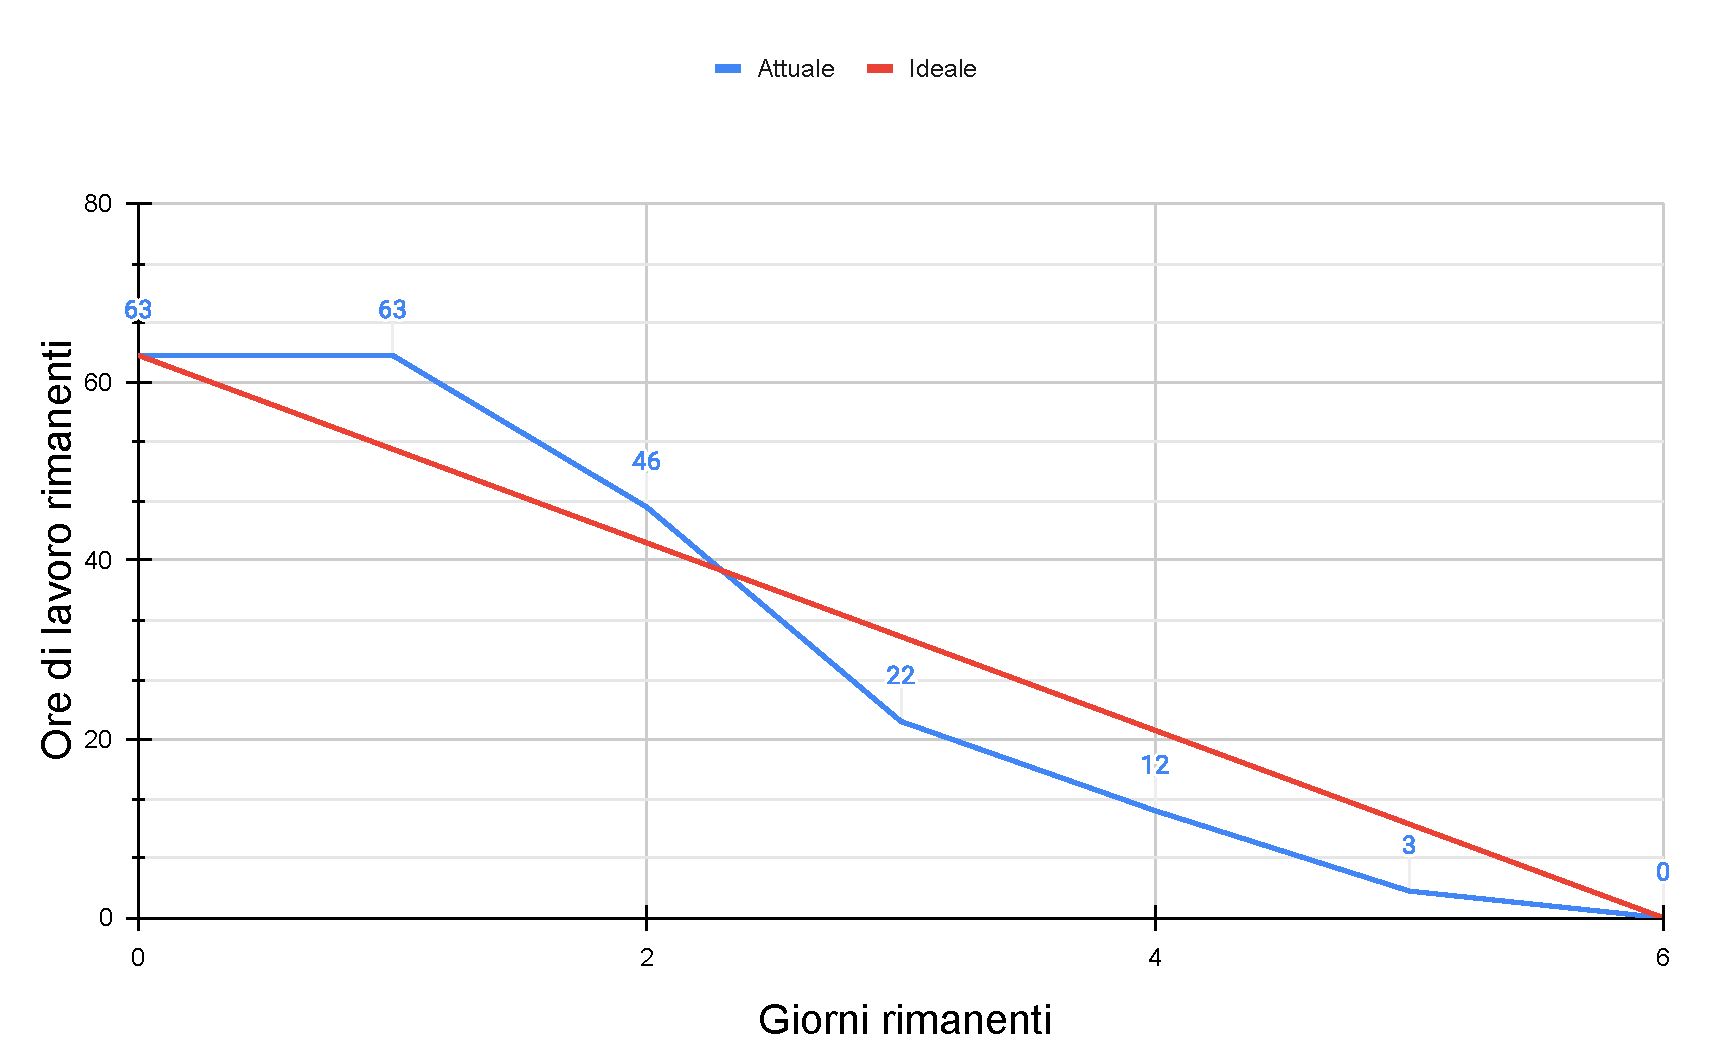
\includegraphics[trim= 0cm 0cm 0cm 0cm, clip, width=1\linewidth]{Deliverables/fourth-deliverable/img/BurndownChart.pdf}
    \caption{Burndown Chart Sprint \#$2$}
\end{figure}






\subsection{Test Case}

\begin{landscape}

\begin{longtable}
{p{0.4cm}|p{2.4cm}|p{0.4cm}|p{2.5cm}|p{3cm}|p{2.5cm}|p{2cm}|p{2.5cm}|p{2.5cm}|p{2cm}}
\caption{Test Cases Design Sprint \#2}\label{tab:TestCasesSprint2} \\
\hline
\textbf{ID} &\textbf{User Story} & \textbf{N.}& \textbf{Descrizione} & \textbf{Dati test case} & \textbf{Precondizioni} & \textbf{Dipendenze}& \textbf{Risultato atteso} & \textbf{Risultato effettivo} & \textbf{Note}  \\
\hline
\endfirsthead

\hline
\textbf{ID} &\textbf{User Story} & \textbf{N.} & \textbf{Descrizione} &\textbf{Dati test case} & \textbf{Precondizioni} & \textbf{Dipendenze}& \textbf{Risultato atteso} & \textbf{Risultato effettivo} & \textbf{Note}  \\
\hline
\endhead


\multirow{19}{0.2cm}{14} & \multirow{19}{0.2cm}{Inserimento prodotto} 
& 1 & Il produttore autenticato inserisce un prodotto & Vai al login del portale, inserisci: email e password, nella pagina clicca su l'icona + e inserisci tutti i dati richiesti & email e password devono esistere nel database& & Il nuovo prodotto deve essere presente lato database. Il produttore visualizza la lista aggiornata& Il prodotto viene inserito correttamente nel database& \\

&& 2 & Il produttore autenticato inserisce un prodotto e non fornisce i dati obbligatori richiesti & Vai al login del portale, inserisci: email e password, nella pagina clicca su l'icona + e non inserire i dati obbligatori  & email e password devono esistere nel database& & Il prodotto non viene inserito nel database e il produttore viene avvisato con un banner dell'errore& il bottone salva non viene attivato& \\

&& 3 & Il produttore autenticato inserisce un prodotto e inserisce un prezzo negativo & Vai al login del portale, inserisci: email e password, nella pagina clicca su l'icona + e inserisci un prezzo negativo & email e password devono esistere nel database& & Il prodotto non viene inserito nel database e il produttore viene avvisato con un banner dell'errore& il bottone salva non viene attivato& \\

&& 4 & Il produttore autenticato inserisce un prodotto e inserisce una quantità negativa & Vai al login del portale, inserisci: email e password, nella pagina clicca su l'icona + e inserisci un quantità negativa & email e password devono esistere nel database& & Il prodotto non viene inserito nel database e il produttore viene avvisato con un banner dell'errore& il bottone salva non viene attivato& \\

\hline
\hline
\newpage


\multirow{13}{0.2cm}{1} & \multirow{13}{0.2cm}{Registrazione cliente - produttore} 

& 5 & Il cliente può registrarsi alla piattaforma & Vai al login del portale, seleziona registrati come cliente, inserisci: username, email e password & l'email NON deve essere già presente nel database& & Il cliente viene registrato e viene inserito sia su MongoDB sia su Firebase& il nuovo cliente viene registrato sia lato mongoDB sia Firebase e gli viene assegnato il ruolo& \\

&& 6 & Il produttore può registrarsi alla piattaforma & Vai al login del portale, seleziona registrati come azienda, inserisci tutti i dati richiesti & l'email NON deve essere già presente nel database& & Il produttore viene registrato sia su MongoDB sia su Firebase& il nuovo produttore viene registrato sia lato mongoDB sia Firebase e gli viene assegnato il ruolo& \\

&& 7 & Il cliente si registra con una mail non valida& Vai al login del portale, seleziona registrati come cliente, inserisci una email errata (non compare @ e/o il dominio) &  & & Viene mostrato un banner di email non valida& Mostrato il messaggio di email non è valida& \\

&& 8 & Il produttore si registra con una mail non valida& Vai al login del portale, seleziona registrati come azienda, inserisci una email errata (non compare @ e/o il dominio) &  & & Viene mostrato un banner di email non valida& Mostrato il messaggio di email non è valida& \\

&& 9 & Il cliente si registra con una mail già esistente& Vai al login del portale, seleziona registrati come cliente, inserisci una email già presente&  & & Viene mostrato un banner di email precedentemente inserita& Mostrato il messaggio di email è già in uso& \\

&& 10 & Il produttore si registra con una mail già esistente& Vai al login del portale, seleziona registrati come azienda, inserisci una email già presente&  & & Viene mostrato un banner di email precedentemente inserita& Mostrato il messaggio di email è già in uso& \\

&& 11 & Il cliente si registra ma lascia vuoto uno o più campi obbligatori& Vai al login del portale, seleziona registrati come cliente, e lascia vuoto uno o più campi&  & & Viene mostrato un banner di errore& Mostrato un messaggio indicate il relativo campo mancante & \\

&& 12 & Il produttore si registra ma lascia vuoto uno o più campi obbligatori& Vai al login del portale, seleziona registrati come cliente, e lascia vuoto uno o più campi&  & & Viene mostrato un banner di errore& Mostrato un messaggio indicate il relativo campo mancante& \\

\hline
\hline
\newpage

\multirow{17}{0.2cm}{2} & \multirow{17}{0.2cm}{Autenticazione cliente - produttore} 

& 13 & Il cliente può autenticarsi sulla piattaforma & Vai al login del portale inserire email e password& Il cliente deve essersi precedentemente registrato& & Il cliente viene autenticato e riportato alla schermata home & Viene riportato nella schermata degli ordini&\\

&& 14 & Il produttore può autenticarsi sulla piattaforma & Vai al login del portale, seleziona registrati come azienda, inserisci tutti i dati richiesti & Il produttore deve essersi precedentemente registrato& & Il produttore viene autenticato e riportato alla sua schermata dedicata& Viene portato nella sua dashboard dedicata& \\

&& 15 & Il cliente tenta il login senza inserire l'email & Vai al login del portale, lascia vuoto il campo email, inserisci una password, premi 'Accedi'& Il cliente è registrato con una password nota&&  Il sistema mostra un messaggio di errore indicando che l'email è obbligatoria e non esegue l'autenticazione& Viene mostrato un messaggio di email non valida&\\

&& 16 & Il cliente tenta il login senza inserire la password & Vai al login del portale, inserisci un'email valida, lascia vuoto il campo password, premi 'Accedi'& Il cliente è registrato con un'email nota&&  Il sistema mostra un messaggio di errore indicando che la password è obbligatoria e non esegue l'autenticazione& Viene mostrato un messaggio di errore durante il login&\\

&& 17 & Il cliente tenta il login con un'email non valida (formato errato) & Vai al login del portale, inserisci un'email con formato non valido (non compare @ e/o il dominio), inserisci una password, premi 'Accedi'& && Il sistema mostra un messaggio di errore indicando che il formato dell'email non è valido e non esegue l'autenticazione & Viene mostrato un messaggio di email non valida&\\

&& 18 & Il cliente tenta il login con email valida ma password errata & Vai al login del portale, inserisci un'email registrata e una password errata, premi 'Accedi'& Il cliente è registrato con l'email inserita ma con una password differente&& Il sistema mostra un messaggio di errore e non esegue l'autenticazione& Viene mostrato un messaggio di errore durante il login&\\


&& 19 & Il cliente tenta il login con un'email non registrata & Vai al login del portale, inserisci un'email non presente nel sistema e una password qualsiasi, premi 'Accedi'& L'email inserita non corrisponde a nessun utente registrato&& Il sistema mostra un messaggio di errore e non esegue l'autenticazione&  Viene mostrato un messaggio di errore durante il login&\\


&& 20 & Il produttore tenta il login senza inserire l'email & Vai al login del portale (sezione azienda), lascia vuoto il campo email, inserisci una password, premi 'Accedi'& Il produttore è registrato con una password nota&&  Il sistema mostra un messaggio di errore indicando che l'email è obbligatoria e non esegue l'autenticazione& Viene mostrato un messaggio di email non valida&\\


&& 21 & Il produttore tenta il login senza inserire la password & Vai al login del portale (sezione azienda), inserisci un'email valida, lascia vuoto il campo password, premi 'Accedi'& Il produttore è registrato con un'email nota&&  Il sistema mostra un messaggio di errore indicando che la password è obbligatoria e non esegue l'autenticazione& Viene mostrato un messaggio di errore durante il login&\\

&& 22 & Il produttore tenta il login con un'email non valida (formato errato) & Vai al login del portale (sezione azienda), inserisci un'email con formato non valido (non compare @ e/o il dominio), inserisci una password, premi 'Accedi'& Nessuna specifica, il controllo è sul formato&&  Il sistema mostra un messaggio di errore indicando che il formato dell'email non è valido e non esegue l'autenticazione& Viene mostrato un messaggio di email non valida&\\

&& 23 & Il produttore tenta il login con email valida ma password errata & Vai al login del portale (sezione azienda), inserisci un'email registrata e una password errata, premi 'Accedi'& Il produttore è registrato con l'email inserita ma con una password differente&&  Il sistema mostra un messaggio di errore "Email o password non validi" (o simile) e non esegue l'autenticazione& Viene mostrato un messaggio di errore durante il login&\\

&& 24 & Il produttore tenta il login con un'email non registrata & Vai al login del portale (sezione azienda), inserisci un'email non presente nel sistema e una password qualsiasi, premi 'Accedi'& L'email inserita non corrisponde a nessun produttore registrato&&  Il sistema mostra un messaggio di errore "Email o password non validi" (o simile, per non rivelare se l'email esiste) e non esegue l'autenticazione& Viene mostrato un messaggio di errore durante il login&\\

\hline
\hline

\newpage
\multirow{6}{0.2cm}{14} & \multirow{6}{0.2cm}{Inserimento prodotto} 

& 25 & Eliminazione di un prodotto & Con Jest inviare una richiesta di Delete di un prodotto inserendo un identificativo & L'identificativo deve essere presente nel database& & Messaggio di successo da parte del endpoint della API e eliminazione lato database & Test superato & \\

&& 26 & Eliminazione di un prodotto inesistente & Con Jest inviare una richiesta di Delete di un prodotto inserendo un identificativo & L'identificativo non deve essere presente nel database& & Messaggio di errore da parte del endpoint della API & Test superato & \\

\hline
\hline
\newpage

\multirow{7}{0.2cm}{20} & \multirow{7}{0.2cm}{Aggiornamento prodotto} 

& 27 & Inserimento di un prodotto & Con Jest inviare una richiesta di creazione di un prodotto inserendo tutti i campi necessari& L'identificativo del produttore deve essere già presente nel database  &&  Messaggio di successo da parte del endpoint della API e creazione del prodotto lato database& Test superato & \\

&& 28 & Inserimento di un prodotto prodotto lasciando vuoti i campi obbligatori & Aprire Jest e inviare una richiesta di creazione di un prodotto lasciando vuoti i campi obbligatori (es. nome produttore) &&&Messaggio di errore da parte del endpoint della API & Test superato & \\

\hline
\hline

\multirow{3}{0.2cm}{5} & \multirow{3}{0.2cm}{Ricerca prodotti} 

& 29 & Ricerca prodotti & Da interfaccia grafica utilizzare i filtri messi a disposizione per la ricerca &&&  Vedere se i dati a schermo sono stati filtrati correttamente& Test superato & \\

\hline
\hline

\multirow{2}{0.2cm}{6} & \multirow{2}{0.2cm}{Ricerca produttore} 

& 30 & Ricerca produttore & Da interfaccia grafica utilizzare cerca produttore &&&  Vedere se i dati a schermo sono stati filtrati correttamente& Test superato & \\

\hline
\hline


\end{longtable}


\end{landscape}
\restoregeometry


\subsection{Sprint Review}

Durante la Sprint Review del secondo sprint del progetto Agritrento, sono state presentate e valutate le funzionalità sviluppate rispetto agli obiettivi definiti nello Sprint Planning.

Funzionalità completate e mostrate:
\begin{itemize}
    \item Implementazione di una migliore UI
    \item Gestione dei ruoli lato firebase e mongoDB
    \item Ricerca prodotti e produttori
    \item Creazione di un carrello
    \item Creazione di un ordine composto da più prodotti, eseguibile solo da un cliente
    \item Dashboard lato produttore dove può aggiornare e vedere la disponibilità dei propri prodotti
    \item Dashboard lato amministratore, solo UI, dove può vedere delle segnalazioni, le notifiche e gestire i produttori
    \item Implementazione di endpoint autenticati (Rimuovi prodotto, crea prodotto, rimuovi ordine, crea ordine,  ecc. lato cliente e produttore) dove viene verificato che chi manda il token JWT abbia un ruolo coerente con l'azione che vuole eseguire.
    \item Inserimento delle immagini per i prodotti più comuni
    \item Recupero della password di un utente
\end{itemize}

Il team ha riconfermato la stabilità delle vecchie API V1 e già alcune sono state sostituite con la V2 che richiede l'autenticazione. 

I prossimi sviluppi sarebbero quelli di :
\begin{itemize}
    \item Introdurre la paginazione, già presente ma non funzionante ancora.
    \item Aggiungere nuovamente le quantità dei prodotto nel caso un cliente eliminasse l'ordine
    \item Introdurre un metodo di pagamento in app
    \item Iniziare a far conoscere l'applicazione ai produttori locali
    \item Introdurre nella dashboard produttore la possibilità di accettare o rifiutare l'ordine
\end{itemize}

\vspace{0.5cm}

\subsection*{Product Backlog Refinement}
Il meeting di raffinamento ha permesso di riallineare le priorità e ottimizzare la pianificazione in base agli sviluppi dello Sprint 2.


\textbf{Incontro di raffinamento backlog:}

Durante il Product Backlog Refinement il team non ha trovato User Story da eliminare o inserire.

\vspace{0.5cm}

\subsection{Sprint Retrospective}

\textbf{Conclusioni e osservazioni:}
\begin{itemize}
    \item \textbf{Cosa ha funzionato:} In generale c'è stata una collaborazione da parte di tutti i membri del team.
    
    \item \textbf{Cosa non ha funzionato:} Ribadiamo quanto scritto nello sprint precedente, ovvero di una documentazione a tratti molto pesante e noiosa. La gestione del tempo per via degli esami prima della deadline del D4 ha rallentato un po' il progetto, ma dato che volevamo presentare l'applicazione il più completa possibile abbiamo continuato a lavorare intensamente nonostante le tempistiche ridotte.
    
    \item \textbf{Adozione di pratiche Agile:} Ci è capitato di ritrovarci per programmare tutti assieme e soprattutto per avere consigli dagli altri membri del team.
    
    \item \textbf{Dinamiche di gruppo:} abbiamo notato ancora una buona disponibilità del team, nonostante i vari impegni per quanto riguarda tirocini, tesi, lavoro, studio, ecc.
    
    \item \textbf{Spunti per il prossimo Sprint:}
    \begin{itemize}
        \item Implementazione pagamento.
        \item Implementazione delle notifiche, segnalazioni e valutazione del produttore da parte del cliente.
        \item Rendere utilizzabile la dashboard del amministratore.
    \end{itemize}
\end{itemize}
\subsection{Architettura di Progetto e Stack Tecnologico utilizzato}
Per lo sviluppo del nostro progetto abbiamo implementato un'architettura client-server con comunicazione RESTful. La soluzione è strutturata nei seguenti componenti:

\subsubsection*{Frontend}
    \begin{itemize}
    \item Vue.js 3, framework JavaScript progressivo per la costruzione di interfacce utente moderne e reattive
    \end{itemize}
    
\subsubsection*{Backend}
    \begin{itemize}
    \item Node.js, ambiente di runtime JavaScript lato server
    \item Express, framework web minimale e flessibile per la gestione delle richieste HTTP e la definizione delle API
    \item MongoDB, database NoSQL orientato ai documenti per la persistenza dei dati
    \item Firebase Authentication per la gestione delle registrazioni e degli accessi
    \item Jest per l'implementazione dei test delle API
    \end{itemize}
    
\subsubsection*{Strumenti di sviluppo}
    \begin{itemize}
    \item Axios per gestire le chiamate HTTP tra client e server
    \item MongoDB Compass per la visualizzazione e manipolazione diretta dei dati
    \item GitHub per il controllo di versione e la collaborazione nel team
    \item Postman per il test delle chiamate API, in più rispetto a Jest
    \item Visual Studio Code come ambiente di sviluppo integrato
    \end{itemize}

\subsection{Diagramma del deploy finale}

\begin{figure}[h!]
    \centering
    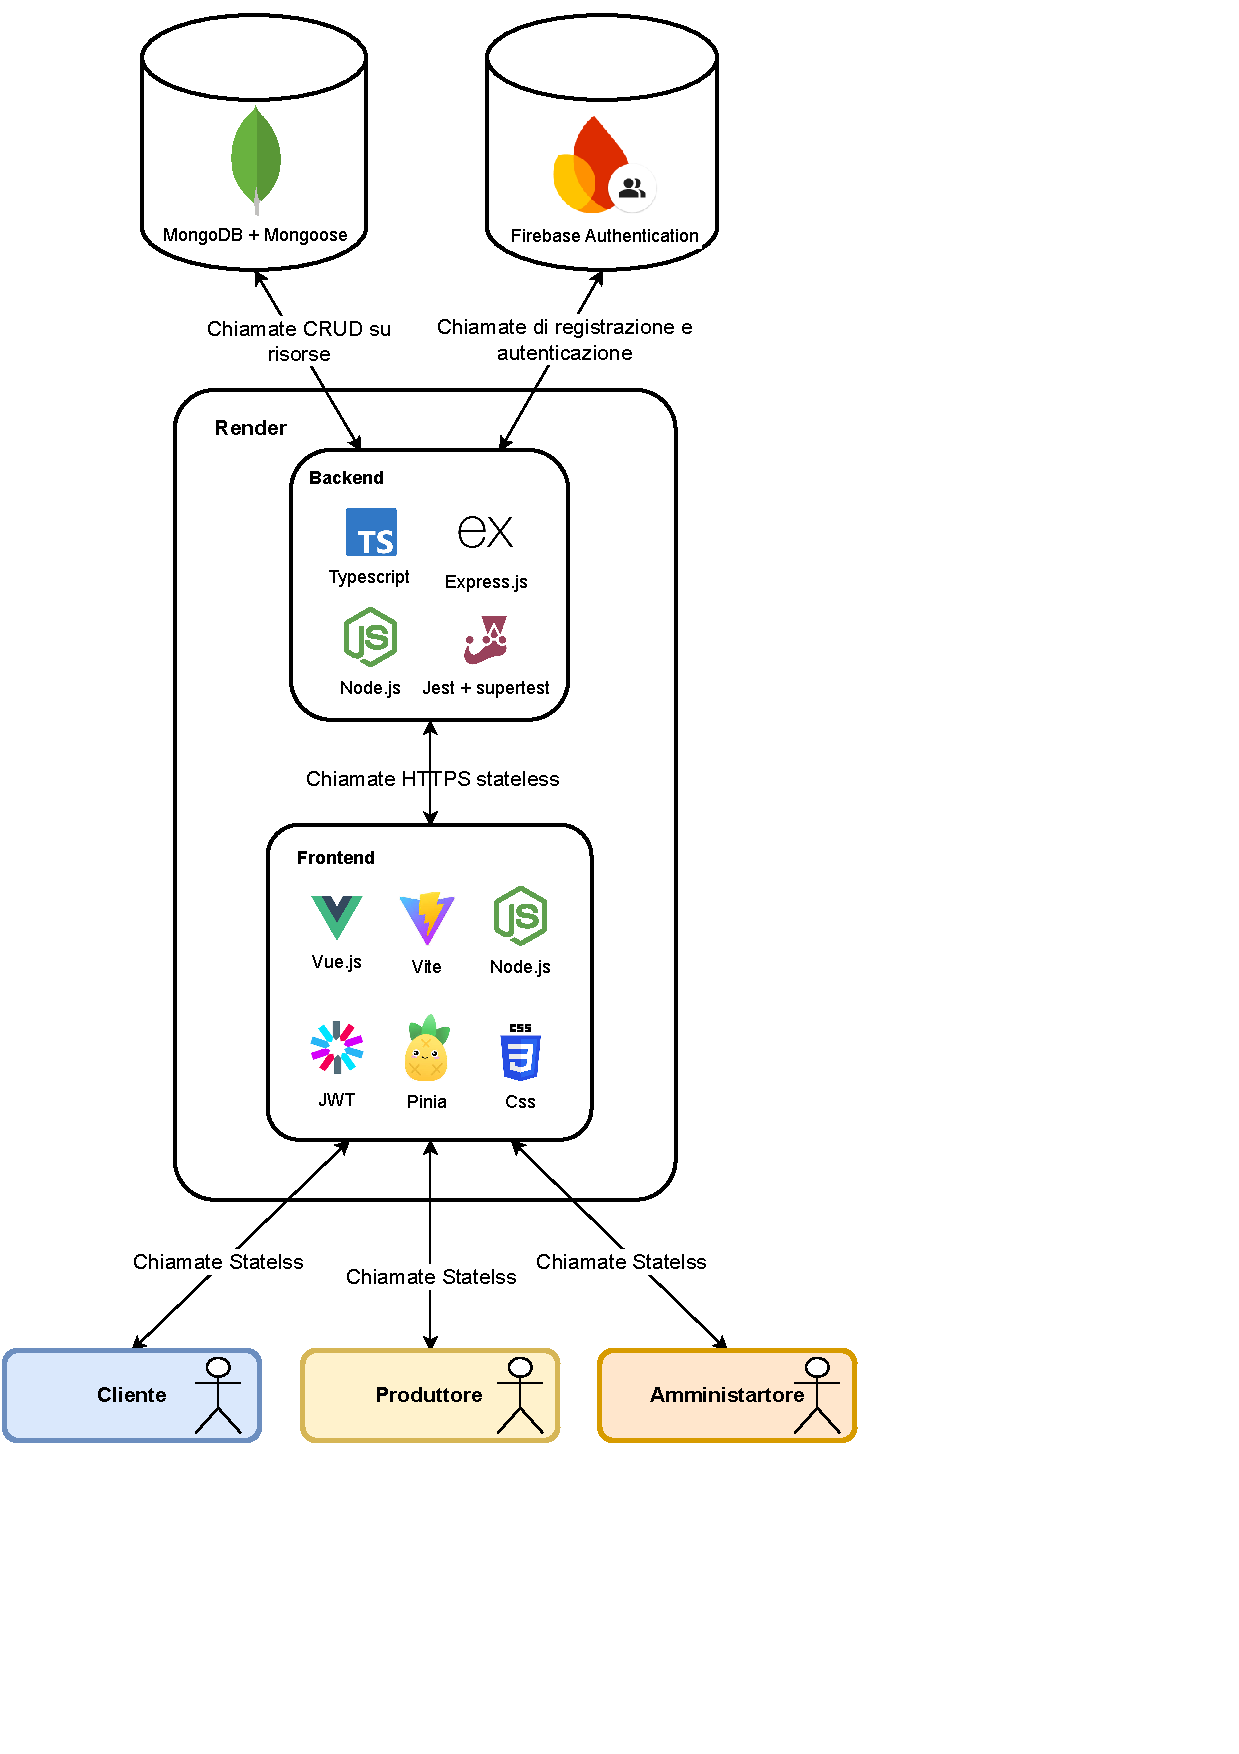
\includegraphics[trim= 0cm 5cm 6.5cm 0cm, clip, width=0.8\linewidth]{Deliverables/fourth-deliverable/img/DiagrammaAgriTrento.drawio.pdf}
    \caption{Deploy finale di AgriTrento}
\end{figure}

\newpage
\subsection{Conclusioni}

Con questo progetto abbiamo imparato davvero molte cose, dall'utilizzare GitHub in un ambiente collaborativo di Team al capire come funziona \verb|Node.js| con il suo Packet manager \verb|npm| fino al Deployment su una piattaforma apposita quale Render.


Sarebbe stato interessante affrontare anche il tema del deploy di container su servizi di orchestrazione quali Google Cloud o altri, ma visto il poco tempo a disposizione sarebbe diventato un ulteriore livello di complicazione considerando che il corso ha durata di soli 6 mesi.

\vspace{0.5cm}

Inoltre, abbiamo acquisito una comprensione approfondita di cosa significhi lavorare in un team composto da più persone: saper conciliare gli impegni e le esigenze di tutti i membri, distribuire efficacemente i compiti e utilizzare framework di sviluppo come l'approccio Agile.
Tuttavia, abbiamo anche notato come quest'ultimo possa talvolta risultare impegnativo, specialmente a causa della documentazione accessoria richiesta dal corso, che rallenta la produttività complessiva del team.

\vspace{0.5cm}

Questo corso è stato, a nostro avviso, il più bello di tutta la triennale che lascia, senza ombra di dubbio, molto a livello pratico.

Nonostante questo però è stato davvero impegnativo soprattutto per l'ultimo sprint dove c'è stato richiesto di creare molte cose accessorie, non valutate a livello accademico, quali: il video per il comune e piano economico per i prossimi anni.
Anche lo stesso deploy per noi è stato un po' complicato essendo che l'ambiente Render, anche se visto a lezione, ci ha dato filo da torcere essendo che ogni applicazione è diversa dalle altre.









\end{document}